%!TEX root = main.tex

% % Other geometries: Linf/L1 (similar bounds in the linear case), TV maybe? L2 on inverse of generative model maybe?

The kernel approach from previous sections is well-suited for input spaces~$\mathcal X$ equipped with the Euclidian
distance, thanks to the non-expansiveness property~\eqref{eq:non_expansive} of the kernel mapping.
In the case of linear models, this kernel approach corresponds to using $\ell_2$-regularization by taking a linear kernel.
However, other forms of regularization and geometries can often be useful,
for example to encourage sparsity with an~$\ell_1$ regularizer.
Such a regularization approach presents tight links with robustness to~$\ell_\infty$ perturbations on input data,
thanks to the duality relation $\|w\|_1 = \sup_{\|u\|_\infty} \langle w, u \rangle$~\citep[see][]{xu2009robust}.

In the context of deep networks, we can leverage such insights to obtain new regularizers,
expressed in the same variational form as the lower bounds in Section~\ref{sub:lower_bounds},
but with different geometries on~$\mathcal X$. For $\ell_\infty$ perturbations, we obtain
\begin{equation}
\label{eq:gradient_l1}
\sup_{x, y\in \mathcal X} \frac{f(x) - f(y)}{\|x - y\|_\infty} \quad \geq \quad \sup_{x \in \mathcal X} \|\nabla f(x) \|_1.
\end{equation}
The Lipschitz regularizer (l.h.s.) can also be taken in an adversarial perturbation form, with~$\ell_\infty$-bounded perturbations $\|\delta\|_\infty \leq \epsilon$.
When considering the corresponding robust optimization problem
\begin{equation}
\label{eq:robust_linf}
\min_\theta \frac{1}{n} \sum_{i=1}^n \sup_{\|\delta\|_\infty \leq \epsilon} \ell(y_i, f_\theta(x_i + \delta)),
\end{equation}
we may consider the PGD approach of~\citet{madry2018towards}, or the associated gradient penalty
approach with the~$\ell_1$ norm, which is a good approximation when~$\epsilon$ is small~\citep{lyu2015unified,simon2018adversarial}.
% \begin{equation*}
% % \label{eq:adv_norm_linf}
% \sup_{x \in \mathcal X, \|\delta\|_\infty \leq \epsilon} f(x + \delta) - f(x).
% \end{equation*}

As most visible in the gradient $\ell_1$-norm in~\eqref{eq:gradient_l1}, these penalties encourage some sparsity
in the gradients of~$f$, which is a reasonable prior for regularization on images, for instance, where we might only
want predictions to change based on few salient pixel regions. This can lead to gains in interpretability, as observed by~\citet{tsipras2018there}.
% We push this principle one step further in our experiments, by considering other structured penalties on the gradients
% such as the total variation.

We note that in the case of linear models, our robust margin bound of Section~\ref{sub:guarantees} can be adapted to
$\ell_\infty$-perturbations, by leveraging Rademacher complexity bounds for $\ell_1$-constrained models~\citep{kakade2009complexity}.
Obtaining similar bounds for neural networks would be interesting but goes beyond the scope of this paper.

% \paragraph{Experiments with $\ell_\infty$ adversaries.}
% Figure~\ref{fig:robust_tradeoffs_linf} shows similar curves to Figure~\ref{fig:robust_tradeoffs}
% from Section~\ref{sub:exp_robust}, but where the attacker is constrained in $\ell_\infty$ norm instead
% of $\ell_2$ norm.
% We can see that using the right metric in PGD indeed helps against an~$\ell_\infty$ adversary,
% nevertheless controlling global stability through the RKHS norm as in the~$\|f\|_\delta^2$ and~$\|\nabla f\|^2$
% penalties can still provide some robustness against such adversaries, even with large $\epsilon_test$.
% For gradient penalties, we find that the different geometries behave quite similarly,
% which may suggest that more appropriate optimization algorithms than SGD could be needed to
% better accommodate the non-smooth case of $\ell_1/\ell_\infty$, or perhaps that both algorithms are actually
% controlling the same notion of complexity on this dataset.

% \begin{figure*}[tb]
% 	\centering
% 	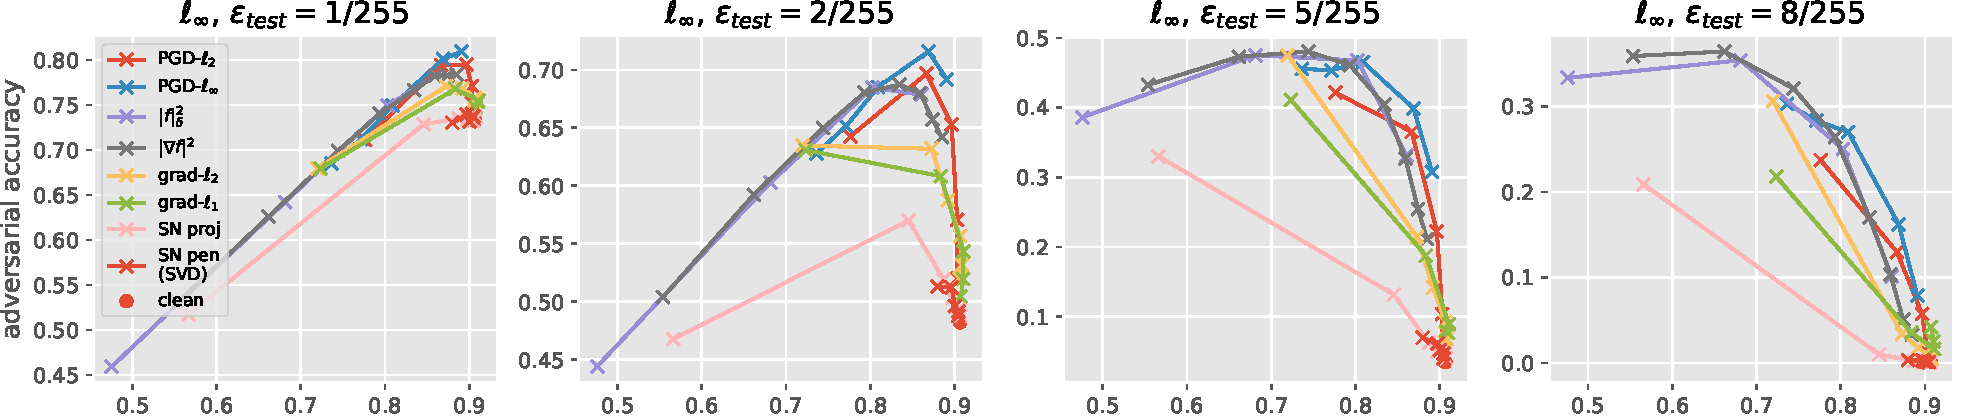
\includegraphics[width=.95\textwidth]{figures/cifar10_vgg/test_vs_adv_linf.pdf}
% 	\caption{$\ell_\infty$ robustness trade-off curves of different regularization methods for VGG11 on CIFAR10.
% 	Each plot shows test accuracy vs adversarial test accuracy
% 	for $\ell_\infty$ bounded 40-step PGD adversaries with a fixed~$\epsilon_{\text{test}}$.
% 	Different points on a curve correspond to training with different regularization strengths,
% 	with the leftmost points corresponding to the strongest regularization.}
% 	\label{fig:robust_tradeoffs_linf}
% \end{figure*}
